\documentclass{article}
%-- coding: UTF-8 --
\usepackage[UTF8]{ctex}
\usepackage[utf8]{inputenc}
\usepackage{geometry}
\geometry{left=3.18cm,right=3.18cm,top=2.54cm,bottom=2.54cm}
\usepackage{hyperref}
\hypersetup{hidelinks,
	colorlinks=true,
	allcolors=black,
	pdfstartview=Fit,
	breaklinks=true}

\usepackage{graphicx} % 引入图片
\usepackage{enumitem} % 取消列表默认间距
\geometry{left=3.18cm,right=3.18cm,top=2.54cm,bottom=2.54cm}
\usepackage{hyperref}
\hypersetup{hidelinks,
	colorlinks=true,
	allcolors=black,
	pdfstartview=Fit,
	breaklinks=true}
\usepackage{listings}
\usepackage{xcolor}
\usepackage{fontspec}
\usepackage{ulem}
\usepackage{array}

% 嵌入代码风格
\lstset{
	language    = c++,
	breaklines  = true,
	captionpos  = b,
	tabsize     = 4,
	columns     = fullflexible,
	commentstyle = \color[RGB]{0,128,0},
	keywordstyle = \color[RGB]{0,0,255},
	basicstyle   = \small\ttfamily,
	stringstyle  = \color[RGB]{148,0,209}\ttfamily,
	rulesepcolor = \color{red!20!green!20!blue!20},
	showstringspaces = false,
}


\title{\textbf{实验零\hspace{1cm}实验准备}}

% \author{黄韦杰\hspace{3.0cm}刘嘉杰 \\ \href{mailto:hwj@hust.edu.cn}{hwj@hust.edu.cn} \hspace{0.8cm} \href{mailto:m202474039@hust.edu.cn}{m202474039@hust.edu.cn}}
\author{
\begin{tabular}{c @{\hspace{5mm}} c}
    黄韦杰 & 刘嘉杰 \\  % 作者名
    \href{mailto:hwj@hust.edu.cn}{hwj@hust.edu.cn} & \href{mailto:m202474039@hust.edu.cn}{m202474039@hust.edu.cn} % 邮箱
\end{tabular}
}
\date{September 2024}

\begin{document}


\maketitle

% \tableofcontents

\section{环境准备}



工欲善其事必先利其器,搭建一个好的开发环境对于我们学习编程来说是至关重要的。不论你使用的是 Windows 、 Mac OS 还是 Linux,我们都推荐使用 \href{https://code.visualstudio.com/}{VS code(Visual Studio code)} 编辑器。它是微软开发的一款开源跨平台编辑器,几乎在任何系统(\href{https://vscode.dev/}{甚至网页上})编辑任何语言的代码,同学们可以将它理解为一个带有渲染功能的「记事本」。得益于其活跃的社区,VS code 拥有非常丰富的插件,这些插件也使得我们编码体验变得更加友好。

在此说明一下,大家也可以使用 DEV C++、Code Blocks、Visual Studio、Clion、Sublime 等编辑器或编译器,但总体来说,更推荐使用 VS Code。另外,我们每次实验提供的基础代码框架也都是基于 VS Code 给出,同学们需要在此基础上完成实验。

由于本文的篇幅原因,详细的安装步骤放置在这里:\href{https://www.yuque.com/docs/share/86719be1-1e00-45d5-a96e-689d2ef10642?#hwgZt}{\textcolor{blue}{VS Code 安装配置 C++ 教程}}


\subsection{Windows}

\noindent Windows 系统环境安装步骤总体如下:
\begin{enumerate}
    \item 下载 VS Code 并安装(前往 \href{https://code.visualstudio.com/Download}{\textcolor{blue}{https://code.visualstudio.com/Download}} 下载或参考详细安装步骤中的链接)
    \item 下载 MinGW(前往 \href{https://www.mingw-w64.org/downloads/}{\textcolor{blue}{https://www.mingw-w64.org/downloads/}} 下载或参考详细安装步骤中的链接)
    \item 配置环境变量(将 \texttt{g++.exe} 所在目录,配置到 path 环境变量中,\textbf{详细步骤见:}\href{https://www.yuque.com/docs/share/86719be1-1e00-45d5-a96e-689d2ef10642?#hwgZt}{\textcolor{blue}{VS Code 安装配置 C++ 教程}}),确保可以在 cmd 中可以运行 \texttt{g++ --version} 命令
    \item 安装 VS Code 插件,配置 VS Code 中项目运行环境,给Code Runner插件\textbf{添加编译选项 \texttt{--std=c++17}}
\end{enumerate}

\subsection{Mac OS}
\noindent Mac OS中的安装过程与 Windows 类似:
\begin{enumerate}
    \item 使用命令: \texttt{brew install gcc} 安装 gcc 或使用命令: \texttt{xcode-select --install} 安装 xcode 工具集(如果 terminal 可以成功调用 \texttt{g++ --version} ,请忽略该步骤)
    \item 下载安装 VS Code(\href{https://code.visualstudio.com/Download}{\textcolor{blue}{https://code.visualstudio.com/Download}})
    \item 安装 VS Code 插件,配置 VS Code 中项目运行环境,给Code Runner插件\textbf{添加编译选项 \texttt{--std=c++17}}
\end{enumerate}

环境配置是一件非常繁琐且无聊的工作,因为一点小错误就耽误大半个甚至数个小时的情况并不少见,所以希望大家在配置环境的过程中,能够仔细的核对操作的每一步。

如果你不是很幸运,配置过程中出现了与预期不符的情况,并且网上也找不到有效的处理办法,那么请及时联系助教老师帮忙. (\^{}-\^{})

\section{编程语言准备}
尽管编程语言与算法知识并不直接相关,但是为了更好的完成课程教学,统一使用一门语言是非常有必要的。本实验课程需要大家使用 C++ 完成,如果你对 C++ 不是很熟悉,也不必担心,\textbf{我们希望你能够专注到算法和数据结构层面},因此提供了相对完善的实验框架,\textbf{通常只需要你实现若干个函数接口,而不需要关注过多的C++的细节}。当然,对于C++基础的顺序、判断、循环结构以及一些语法特性以及少量容器的使用方法,还是需要你提前掌握的,下面附上了我们认为完成本门课程的实验至少需要了解的内容。另外,每节lab可能会根据需要在实验文档后面补充完成该节lab需要额外了解的C++用法,请大家关注。\\

\noindent {一些需要掌握的 C++ 知识点(粗体为我们认为容易出现错误且难以debug的语法细节):}

\begin{enumerate}
    \item 基本变量类型、变量的定义和使用、\textbf{变量的初始化以及默认值}
    \item if-else, while,for 等基本流程控制语句(\textbf{为什么我的程序卡死了:死循环})
    \item 变量的作用域(\textbf{全局变量和局部变量})
    \item 结构体的定义和使用
    \item 函数的基本使用、函数传参类型(\textbf{在函数中对传入的参数做修改为什么不起作用:值传递、引用传递})、函数的返回
    \item 指针的创建和使用(\textbf{为什么出现segmentation fault:野指针和空指针})
    \item Class 的基本概念(私有、共有,成员变量、成员函数等)
    \item 什么是STL、怎么引入STL的头文件、vector的使用、string的使用
\end{enumerate}

\noindent 参考文档:

\begin{itemize}
    \item cppreference: \href{https://zh.cppreference.com/}{\textcolor{blue}{https://zh.cppreference.com/}}
    \item C语言中文网:\href{http://c.biancheng.net/cplus/}{\textcolor{blue}{http://c.biancheng.net/cplus/}}
    \item 菜鸟文档:\href{https://www.runoob.com/cplusplus/cpp-tutorial.html}{\textcolor{blue}{https://www.runoob.com/cplusplus/cpp-tutorial.html}}
\end{itemize}


在后期实验过程中,同学们遇到任何问题,请首先自己尝试,通过网络搜索,发到群里大家一起讨论,最终考虑求助助教。

\section{小试牛刀:算法世界的初体验}
\subsection{说明}
本次lab的内容旨在让大家熟悉C++语法、熟悉本门课程的实验课流程以及实现方式,\textcolor{red}{本次实验不需要提交任何结果,也不会计入成绩}。本门课程后续的上机实验课程,都会按照类似于本次lab形式进行。

\subsection{实验内容}
当你披荆斩棘\sout{(指安装软件、配置编译环境)},一路来到算法世界的大门口,却发现大门紧闭。无比失望的你突然发现充满古老气息的大门上,有一道谜题:

给你字符串 \texttt{key} 和 \texttt{message} ,分别表示一个加密密钥和一段加密消息。解密 \texttt{message} 的步骤如下:
\begin{enumerate}
    \item 使用 \texttt{key} 中 \texttt{26} 个英文小写字母第一次出现的顺序作为替换表中的字母 顺序 。
    \item 将替换表与普通英文字母表对齐,形成对照表。
    \item 按照对照表 替换 \texttt{message} 中的每个字母。
    \item 空格 ' ' 保持不变。
\end{enumerate}

例如,key = "\textbf{hap}p\textbf{y} \textbf{bo}y"(实际的加密密钥会包含字母表中每个字母 至少一次),据此,可以得到部分对照表('h' -> 'a'、'a' -> 'b'、'p' -> 'c'、'y' -> 'd'、'b' -> 'e'、'o' -> 'f')。

随后,大门不断的循环闪烁显示一组字符串,显然组成了一句话,勇敢的你坚信解开这段话即可打开大门。

\subsection{实验项目结构}

\begin{itemize}[noitemsep]
    \item[$-$] project
        \begin{itemize}[noitemsep]
            \item[$-$] include
                \begin{itemize}[noitemsep]
                    \item[$\bullet$] dessert.hpp
                    \item[$\bullet$] MyEncoder.hpp
                \end{itemize}
            \item[$-$] data
                \begin{itemize}[noitemsep]
                    \item[$-$] sample
                    \item[$-$] generate
                \end{itemize}
            \item[$\bullet$] main.cpp
        \end{itemize}
\end{itemize}

\textbf{project} 文件夹包含了本实验的所有代码源程序以及测试程序。

\textbf{include} 文件夹中,MyEncoder.hpp 定义了 MyEncoder 类,在本实验中,你\textbf{需要且仅需要完成这个类中的\texttt{Encoding}函数},实现解密算法。而desert.hpp文件为测试程序框架,你可以简单地忽略它

\textbf{data} 文件夹中包含针对算法程序正确性测试以及性能测试所需的测试数据以及数据生成器。samples包含了本次实验的测试数据,你可以用文本编辑器(如记事本)打开其中的data.in文件,了解输入形式。另外,generate 包含了测试数据的生成器,你可以简单地忽略它

\textbf{main.cpp} 是正确性检测的主程序,当你编写完 MyEncoder.hpp 后,需要编译运行(或者使用Code Runner运行)main.cpp,测试程序会自动执行。\textcolor{red}{注意:实验中需要运行的文件只有main.cpp生成的可执行文件,如果单独编译运行其他文件可能会出错}。\\


具体的,你需要完成\texttt{MyEncoder.hpp} 中的代码编写:
\begin{lstlisting}
	// @param
	// key: 加密密钥,key仅由小写英文字母及 ' ' 组成,key 包含英文字母表中每个字符('a' 到 'z')至少一次
	// secrets: 待解密的密文数组,secrets中的每一个元素为string类型

	// @return
	// messages: 解密后的消息数组,messages中每一个元素为string类型,与secrets中每个元素一一对应
	vector<string> Encoding(string key, vector<string> secrets) {
		vector<string> messages;
		/* YOUR SOLUTION HERE */
		/* ... */
		return messages;
	}
\end{lstlisting}

完成之后,你可以使用以下的命令或者在vs code中使用Code Runner编译运行\texttt{main.cpp}:
\begin{lstlisting}
        $ g++ --std=c++17 main.cpp
        $ ./a.out(macOS/Linux) 或 a.exe(windows)
\end{lstlisting}

你会看到如下的测试结果,如果显示全部通过,则证明你的算法实现正确。

\begin{figure}[h]
    \centering
    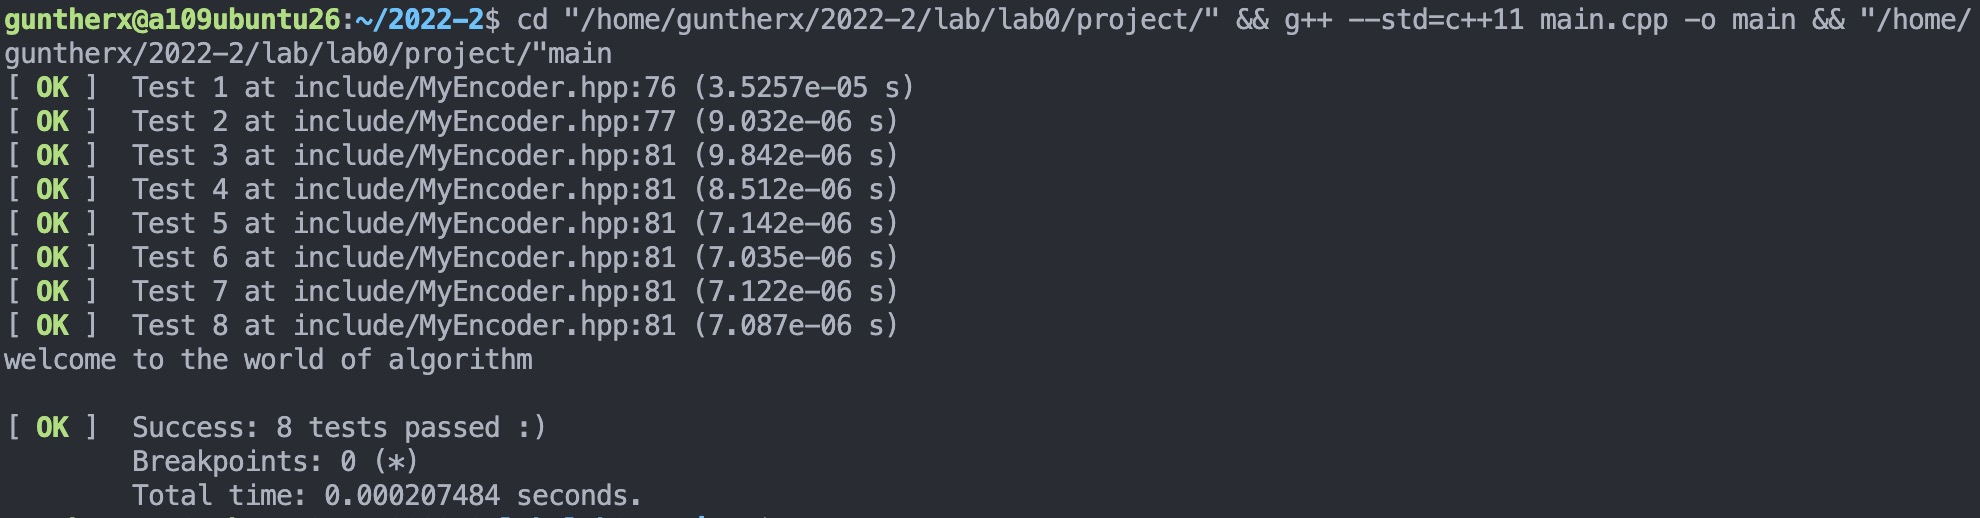
\includegraphics[height=3cm]{img/lab0/lab0-1.png}
\end{figure}

否则,终端命令行会显示你出错的数据和位置,请你根据输出改正。

\end{document}
